\paragraph{ }

It is important to consider many parameters when calculating the orbital decay of a satellite. The most important of these parameters for LEO based constellations is drag. As discussed in other chapters, the drag of a satellite depends on the coefficient of drag, its surface, the density of the air and the velocity at which operates. Solar cycles will directly affect the density of the upper atmosphere. This phenomena is relevant when calculating the drag of the satellite and therefore is essential to compute the orbital decay. \\

Solar cycles are periodic changes in the Sun's activity of approximately 11 years. In each period a solar maximum and minimum can be determined, referring to the amount of periods of sunspot counts. The intensities for these periods vary from cycle to cycle. \\



Different studies have been made throughout the 20th century cycles. In order to understand the change  density of the air changes as consequence of these solar cycles we considered the result data of an old study regarding the 19th solar cycle, which had a duration of 10.5 years between 1958 and 1968. This solar cycle had the highest maximum smoothed sunspot number ever recorded (since 1755), which was of 201.3. This maximum value was recorded in March 1958. This value is high in comparison to other cycles, especially when comparing it to the current 24th solar cycle. In this chapter an analysis will be developed in order to study the influence of the solar cycles on the drag of our satellites. 



\begin{figure}[h]
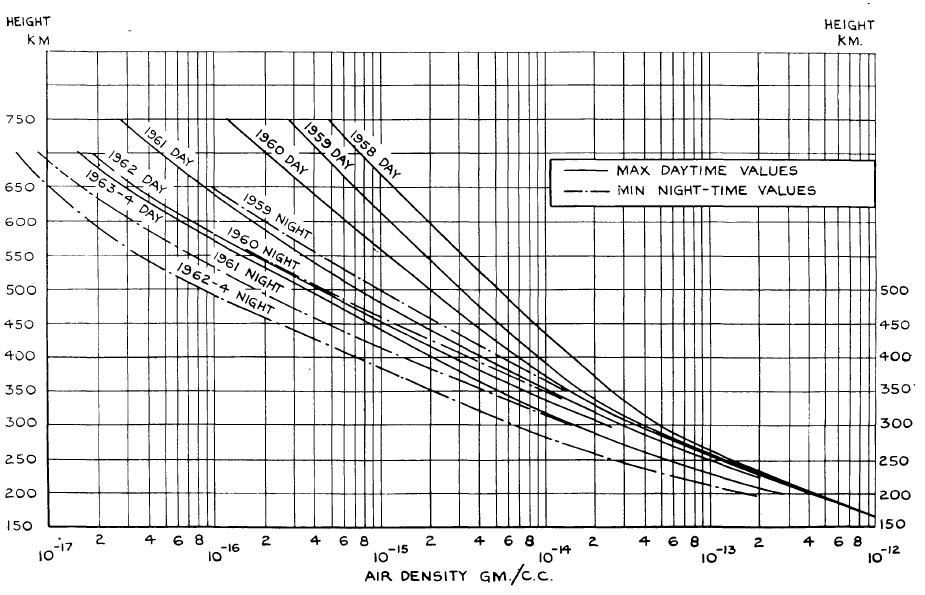
\includegraphics[width=14cm]{solarcycles}
\centering
\caption{Deviation of densities in the upper atmosphere due to the 19th solar cycle}
\end{figure}


At 550 km:

\begin{center}
 \begin{tabular}{||c| c| c||} 
 \hline\hline
Year & D/N & Density at 550km [g/cc]\\ [1ex] 
 \hline
 1958 & Day & 3.2E-14 \\ [1ex]
 \hline
 1958 & Night & 5.0E-15\\[1ex]
 \hline
 1964 & Day & 1.35E-15 \\[1ex]
 \hline
 1964 & Night & 3.35E-16 \\[1ex]
 \hline\hline
%\caption{Density values at solar maximum and minimum of the cycle}
\end{tabular}
\end{center}

These values referring to day and night are the densities of the upper atmosphere at 550 km of altitude respect to the surface of the Earth. The upper atmosphere densities rise during the day following the increase of temperature caused by the radiation of the Sun whereas these values are reduced at night. The orbital decay is on the order of several years whereas these deviations appear every few hours. Thus, in order to compute the orbital decay we will not be taking into account these daily deviations but rather a main value. Therefore the mean density for 1958 will be of 1.85E-14 g/cc and the solar minimum's density of 1964 will be of 8.4E-16 g/cc. \\

In order to analyse how these values may apply to our constellation we first must adjust these - which belong to the 19th solar cycle - to those of the current 24th cycle, which is noticeable less intense. A way of operating this adjustment is comparing the mean solar maximum achieved by each cycle. The maximum monthly smoothed sunspot number of the 19th cycle had a value of 201.3 and a minimum of 9.6 whereas the current 24th ranges between 11.7 and 81.9 approximately. This means that for the 19th cycle a total deviation of 191.7 was measured whilst for the 24th cycle this deviation was only of 70.2. This is crucial if we want to analyse the solar maximum densities.  \\

\begin{figure}[h]
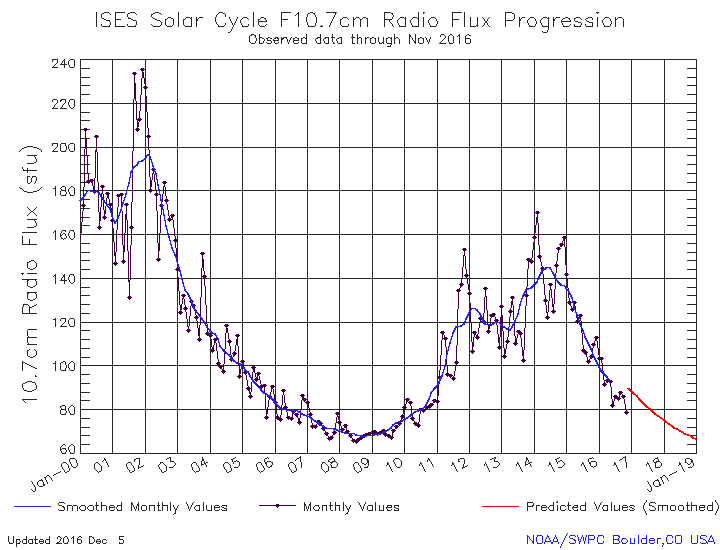
\includegraphics[width=14cm]{24solar}
\centering
\caption{Measured intensities of the 23rd and 24th solar cycles. Source: NOAA}
\label{figure4}
\end{figure}

We must now adjust the mean constant density defined initially to the conditions that this 24th cycle imposes. It is important to note that our satellites will be launched in 2017, and that the 24th cycle is currently decreasing its intensity. Thus, our calculations will be near the conditions of solar minimum, meaning that the drag of our satellite will be smaller than first considered. \\

Our new approach to the density of the atmosphere at 550 km is near the first approximation, but will consider that we are now entering the solar minimum which will remain more or less constant until 2022. As discussed before, the solar minimum represents a singularity with a minimum density of 8.4E-16 g/cc. The approximation taken will be the resulting constant value which represents the mean smoothed densities between 2017 and 2022. \\

The final density at 550 km considering the solar minimum during 2017 to 2022 will be of 2.0E-15 g/cc. 